\chapter{Testování}
\label{sec:Testing}
\vspace{-20pt}
\

V této kapitole je popsáno testování algoritmu optimalizace rychlosti na dráze,
která je popsaná v kapitole~\ref{sec:PlatformControl}, a porovnána s manuálním
řízením i řízením bez optimalizace na základe senzoru..

Pro porovnání potřebujeme spočítat za kolik tiku auto projelo jedno kolo. Tik je
jednotka času, která představuje jeden cyklus časovače. Na to můžeme využít data
bočního zrychlení, která jsou zobrazena na obrázku \ref{fig:Laps}. Levý obrázek je
zrychlením automatického řízení a pravý obrázek je zrychlením manuálního řízení.

\begin{figure}[!h]
    \centering
    \subfloat[Automatické řízení]{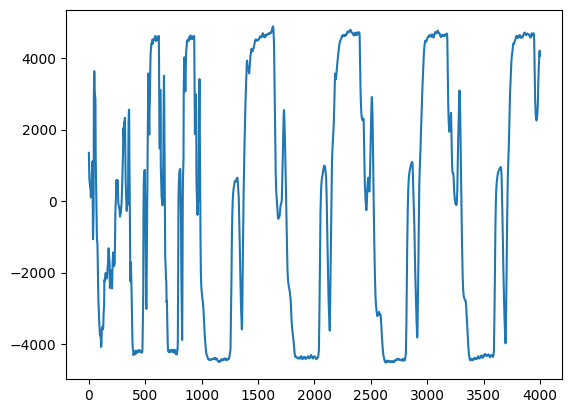
\includegraphics[width = .5\textwidth]{Figures/LapAuto.png}\label{fig:LapsAuto}}
    \subfloat[Manuální řízení]{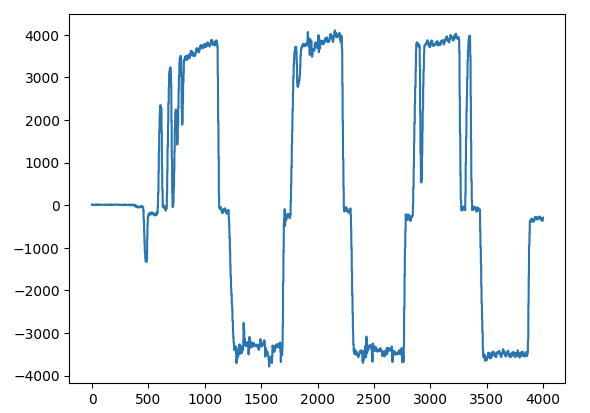
\includegraphics[width = .5\textwidth]{Figures/LapManual.png}\label{fig:LapsManual}}
    \caption{Boční zrychlení během experimentů.}
    \label{fig:Laps}
\end{figure}

Implementace algoritmu prahování zajišťuje pro každý datový bod hodnotu úhlové
rychlosti z~gyroskopu na ose z. Pokud tato hodnota překročí prahovou hodnotu, a
zároveň nebyl ještě zaznamenán polokruh, algoritmus zaznamená časovou známku detekce
jako počátek polokruhu. Polokruh je stav, kdy gyroskop má nejvyšší hodnotu, což z pohledu drahý je jedna ze dvou zatáček. Pokud hodnota úhlové rychlosti klesne pod prahovou hodnotu a
byl již zaznamenán polokruh, znamená to, že byl detekován úplný kruh. Algoritmus
poté zvýší počet detekovaných kol o jednu. Tento proces se opakuje pro každý datový
bod, čímž algoritmus umožňuje sledování a počítání kol na základě úhlové rychlosti
zaznamenané gyroskopem. Použitý algoritmus je ve výpisu:
\begin{lstlisting}[caption = Počet kol, label = lst:countLap]
threshold = 3000
half_lap_detected = False
lap_count = 0
laps = []

for data_point in data:
    if data_point.sensor.gyro.z >= threshold and not half_lap_detected:
        laps.append((lap_count, data_point.timestamp))
        half_lap_detected = True
    elif data_point.sensor.gyro.z <= -threshold and half_lap_detected:
        lap_count += 1
        half_lap_detected = False
\end{lstlisting}

Porovnání automatického s senzory i bez senzoru a manuálního řízení je v tabulce \ref{tab:Comparison}.
\begin{table}[!h]
    \centering
    \begin{tabular}{cccc}
        \hline
        \textbf{Řízení} & \textbf{1 Kolo} & \textbf{2 Kolo} & \textbf{3 Kolo} \\
        \hline
        Automatické s senzory          & 942       & 562 & 343          \\
        Automatické bez senzoru & 1196 & 1175 & 1138 \\
        Manuální 			  & 1178       & 1085 & 1161           \\
        \hline
    \end{tabular}
    \caption{Porovnání manuálního a automatického řízení.}
    \label{tab:Comparison}
\end{table}

Na základě tabulky můžeme vyvodit závěr, že automatické řízení s senzory je rychlejší než automatické řízení bez senzoru. Manuální řízení bylo rychlejší než automatické bez senzoru ale pomalejší než automatické s senzory.
\endinput
